\chapter{Modelo Propuesto} \label{chap:Propuesta}
%parrafo de introduccion recordando objetivo
%La propuesta de este trabajo de tesis consiste en la adopción y adaptación de técnicas y trabajos ya existentes sobre los cuales, realizar las modificaciones que nos permita reconocer rostros en un contexto de vídeo vigilancia.

La propuesta de este trabajo presenta un \textit{pipeline} de reconocimiento de rostros en vídeo donde se usa \ac{EBGM} que ha sido elegido por sus resultado en comparativas realizadas con otros métodos holísticos, y por ser un método que es considerado biométrico por lo expuesto en los capítulos anteriores.

Cabe resaltar que la principal dificultad para su uso en vídeo vigilancia es su necesidad de tener las coordenadas de los ojos ya encontradas para poder determinar el resto de puntos fiduciales. Este hecho es especialmente importante ya que el proceso de estimación de puntos esta ligado a que tipos de modelos se usa y puede ser influenciado por algún patrón dentro de los modelos.

A pesar de la dificultad mencionada, \ac{EBGM} sigue siendo un algoritmo adecuado para el reconocimiento de rostros en vídeo vigilancia. Por ello se propone adoptar el uso de \ac{CLNF} para reemplazar el proceso de estimación de puntos fiduciales que \ac{EBGM} usa.

A continuación se presenta el esquema general de la propuesta de este trabajo de tesis.

\section{Esquema general de la propuesta}
%mostrar y describir las partes del pipe lines de vídeo
Para poder realizar el reconocimiento de rostros en vídeo vigilancia se debe establecer un \textit{pipeline} de procesos para alcanzar dicha meta, a continuación se describe los pasos necesarios para el reconocimiento de rostros:
\begin{enumerate}[label={[\arabic*]}]
\item Realizar la detección de rostros en la escena de vídeo vigilancia.
\item Validar dichas detecciones para descarta falsos positivos.
\item Encontrar puntos fiduciales en el rostro detectado.
\item Aplicar pre-procesamiento a la imagen de rostros detectada.
\item Normalizar imágenes de rostros a un tamaño y posición predefinida.
\item Realizar el proceso de reconocimiento usando \ac{EBGM}.
\item Mostrar el resultado del reconocimiento
\end{enumerate}
En la Figura \ref{im:PropPipeline} se puede observar la lista de procesos o \textit{pipeline} del procedimiento general de la propuesta desde adquisición de la imagen hasta el resultado del reconocimiento.
\begin{figure}[h]
\center
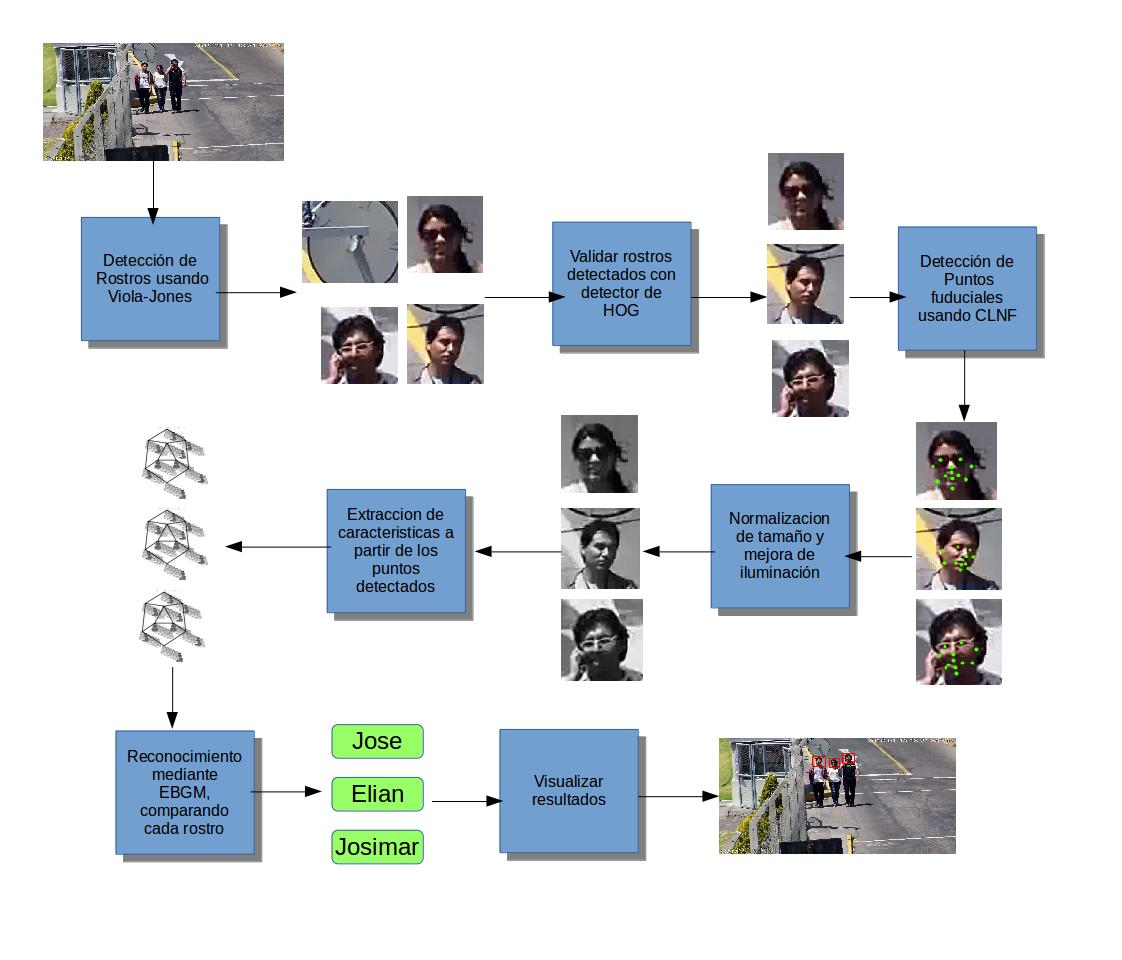
\includegraphics[scale=0.45]{Pipeline}
\caption{\textit{Pipeline} de propuesta, muestra el proceso de reconocimiento de rostros desde la detección en una escena hasta la muestra del resultado.}
\label{im:PropPipeline}
\end{figure}

En el Algoritmo \ref{alg:Propuesta} se describe el funcionamiento de nuestra propuesta donde se trata cada punto relevante:
\begin{algorithm}
\var{names} $\gets$ crear lista para almacenar nombres de imágenes de entrenamiento\;
\var{graphs} $\gets$ crear una lista de \var{FaceGraph}\;
\var{filter} $\gets$ crear un filtro de puntos fiduciales\;
\var{clnf\_model} $\gets$ leer y cargar modelo de entrenamiento para \ac{CLNF}\;
\var{mask} $\gets$ mascaras de Gabor a partir de un conjunto con parámetros\;
\var{trainSet} $\gets$ leer lista de direcciones y nombres de imágenes de entrenamiento\;
\ForEach{\var{element} en \var{trainSet}}
{
	\var{trainIm} $\gets$ leer imagen a partir de \var{element}\;
    \var{success} $\gets$ buscar puntos fiduciales en \var{trainIm} con \var{clnf\_model}\;
    \eIf{\var{success} es cierto}
    {
    	\var{faceLandmarkTrain} $\gets$ asignar lista de puntos fiduciales encontrados con \var{clnf\_model}\;
        añadir nombre de la imagen a la lista \var{names}\;
        \var{graph}$\gets$\textit{ConvertirImagenGrafo}(\var{trainIm},\var{faceLandmarkTrain},\var{mask},\var{filter})\;
    }
    {
    	escribir mensaje de error en entrenamiento\;
    }
}
\If{fuente de vídeo no existe}
{
	escribir mensaje de error en fuente de vídeo y salir de la aplicación\;
}
\While{siempre cierto}
{
	\var{frame} $\gets$ leer desde fuente de vídeo\;
    \var{frameGray} $\gets$ convertir \var{frame} a escala de grises\;
    detectar rostros en \var{frameGray} usando \var{cascade}\;
    \var{faces} $\gets$ guardar coordenadas de rostros detectados por \var{cascade}\;
    \ForEach{\var{element} en \var{faces}}
    {
    	\var{roi} $\gets$ recortar región de rostro en detectada en \var{frameGray} y validar detección con un detector de \ac{HOG}\;
        \var{success} $\gets$ buscar puntos fiduciales en \var{roi} con \var{clnf\_model}\;
    }
    \If{\var{var} es cierto}
    {
    	\var{var} $\gets$ asignar lista de puntos fiduciales encontrados con \var{clnf\_model}\;
        \var{detectedFace} $\gets$ ConvertirImagenGrafo(\var{roi},\var{faceLandmark},\var{mask},\var{filter})\;
    }
    ajustar \var{faceLandmark} a posición real en \var{frame}\;
    dibujar \var{faceLandmark} en \var{frame}\;
    dibujar recuadro de \var{roi} en \var{frame}\;
    \var{name} $\gets$ ReconocerFaceGraph(detectedFace,graphs,names)\;
    dibujar \var{name} sobre recuadro de \var{roi}\;
    visualizar \var{frame}\;
}
\caption{Pipeline de propuesta de reconocimiento de rostros}
\label{alg:Propuesta}
\end{algorithm}


\section{Detección y validación de rostros} 
Para el proceso de detección de rostros se utilizó el algoritmo de Viola-Jones, el cual devuelve regiones donde se detectaron rostros, es conocido que dicho algoritmo funciona bien en imágenes de alta resolución y condiciones de iluminación controladas. Como se observa en la Figura \ref{im:ViolaPerfect}, pero en el contexto de imágenes de vídeo vigilancia las cámara tiene menor resolución y no controlan la condiciones de iluminación, motivo por el cual nos da como resultados regiones que no necesariamente corresponden a un rostro (falsos positivos).

\begin{figure}[h]
\center
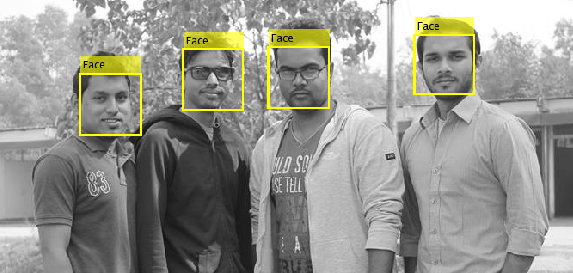
\includegraphics[scale=1]{ViolaPerfect}
\caption{Muestra de una imagen optima detector de Viola-Jones, todos los sujetos observan a la cámara y es una imagen en buena calidad, extraída de Internet}
\label{im:ViolaPerfect}
\end{figure}

Para que la propuesta sea robusta este trabajo presenta un validación mediante el descriptor de \ac{HOG}, de esta manera se mejora el proceso de detección a la vez de validar los resultados del detector de Viola-Jones. En general mejora la detección de rostros en sistemas de vídeo vigilancia.

\subsection{Detector de Viola-Jones}

El proceso de detección comienza con la transformación de la escena al espacio de imagen integral, como es explicado en la Sección \ref{scc:Viola}. Luego se analiza todas las regiones de la escena a través de una ventana para encontrar patrones de características Haar que cumplan con el entrenamiento del clasificador en cascada, dando como resultado las coordenadas de las regiones con rostros detectados. Este proceso se repite por varios tamaños de ventana diferente para detectar rostros en varios tamaños.

Como se observa en la Figura \ref{im:EscenaViola} y \ref{im:EscenaViolaResultados}, Viola-Jones tiene problemas en condiciones de iluminación no controladas, y se puede apreciar claramente que hay varios rostros detectados y un falso positivo. Motivo por el cual es necesario validar con el proceso siguiente.

\begin{figure}[h]
\center
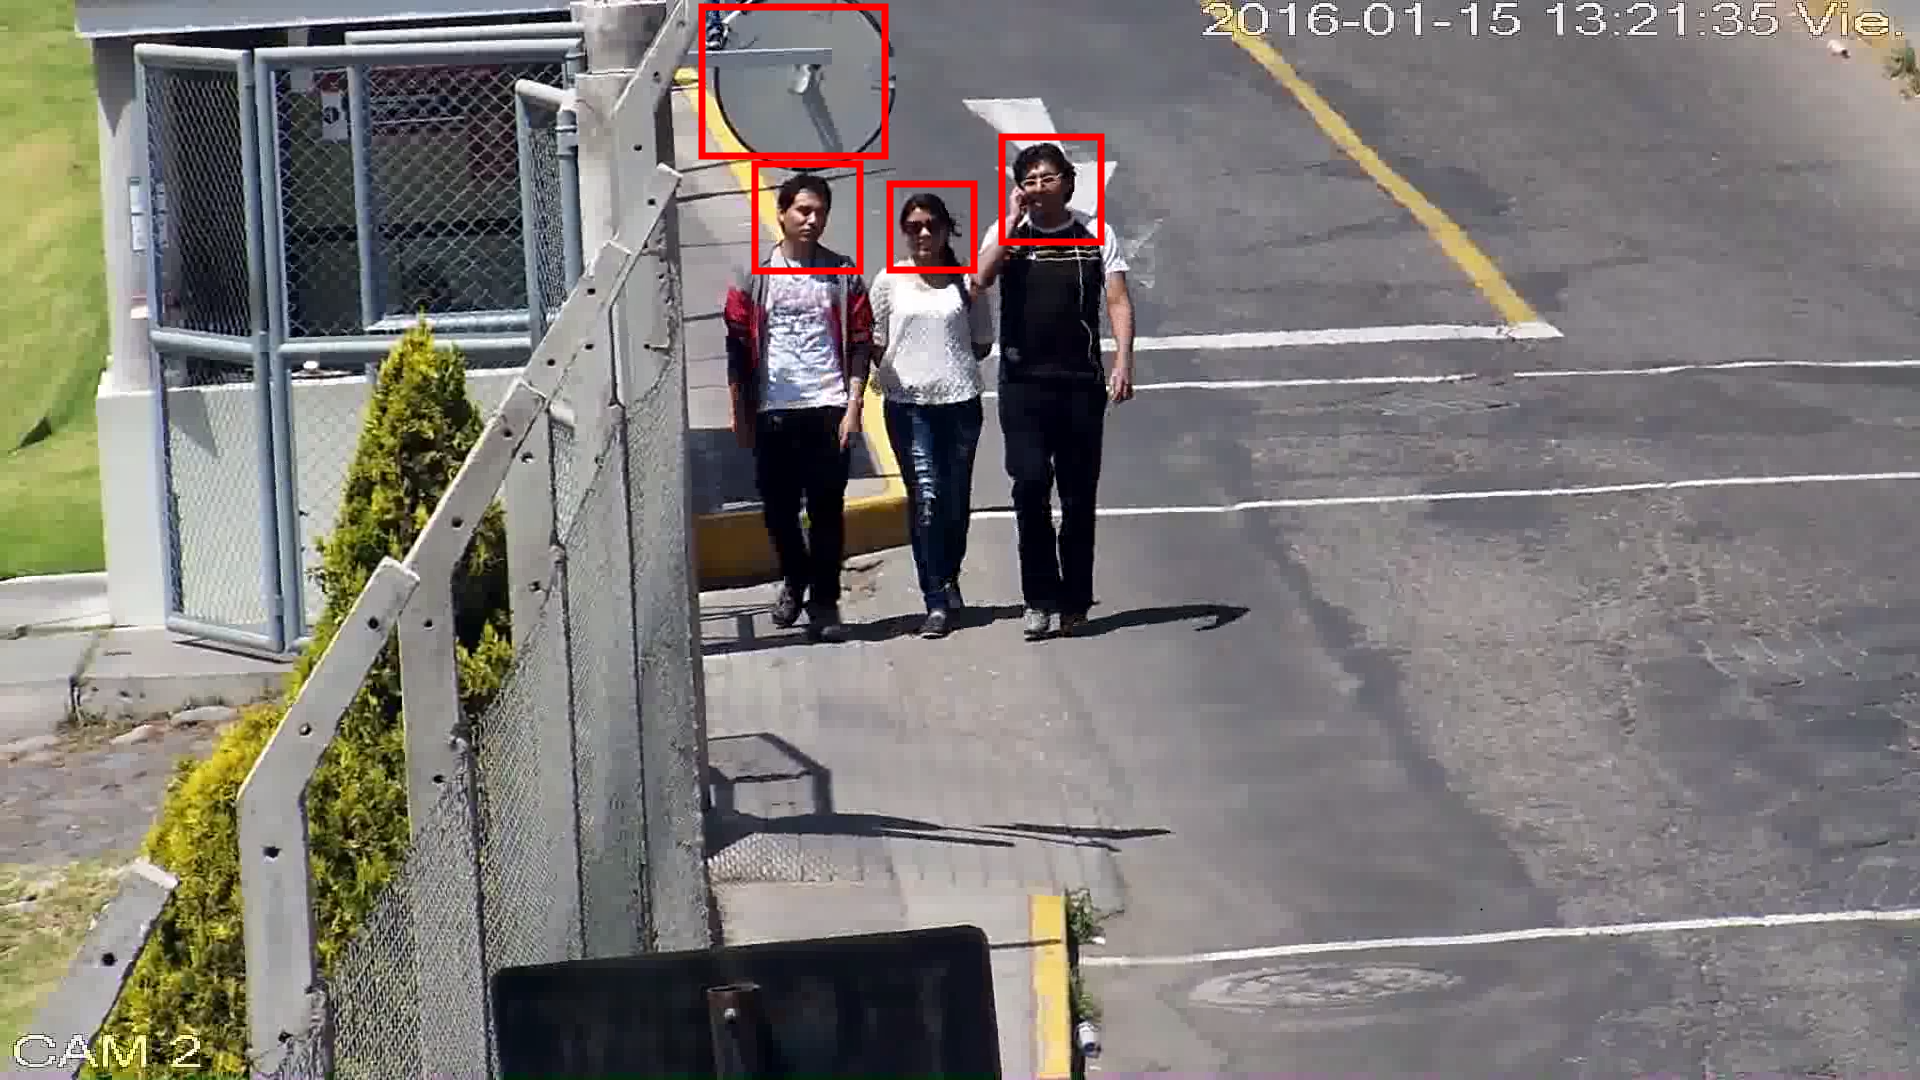
\includegraphics[scale=0.2]{escena_Muestra_error}
\caption{Muestra de  una escena de vídeo vigilancia usando el detector de Viola-Jones}
\label{im:EscenaViola}
\end{figure}

\begin{figure}[h]
\center
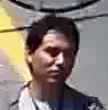
\includegraphics[scale=0.79]{pepe}
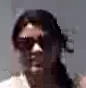
\includegraphics[scale=1]{elian}
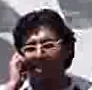
\includegraphics[scale=1]{josimar}
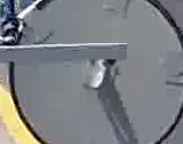
\includegraphics[scale=0.6]{Error}
\caption{Ejemplo de detecciones usando el detector de Viola-Jones, donde la ultima imagen es un falso positivo}
\label{im:EscenaViolaResultados}
\end{figure}

\subsection{Validación con detector de \ac{HOG}}
Para filtrar los falsos positivos que puede entregar el algoritmo de Viola-Jones se propone usar el detector de \ac{HOG} para rostros. %esta elección es motivada por dos razones.

El proceso de detección de rostros usando \ac{HOG} toma una imagen y la trasforma con el descriptor de \ac{HOG} donde se resalta las lineas de contraste y entrega información sobre la gradiente de dicho contraste como se observa en la Figura \ref{im:HOG}

\begin{figure}[h]
\center
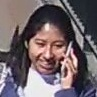
\includegraphics[scale=1.5]{face}
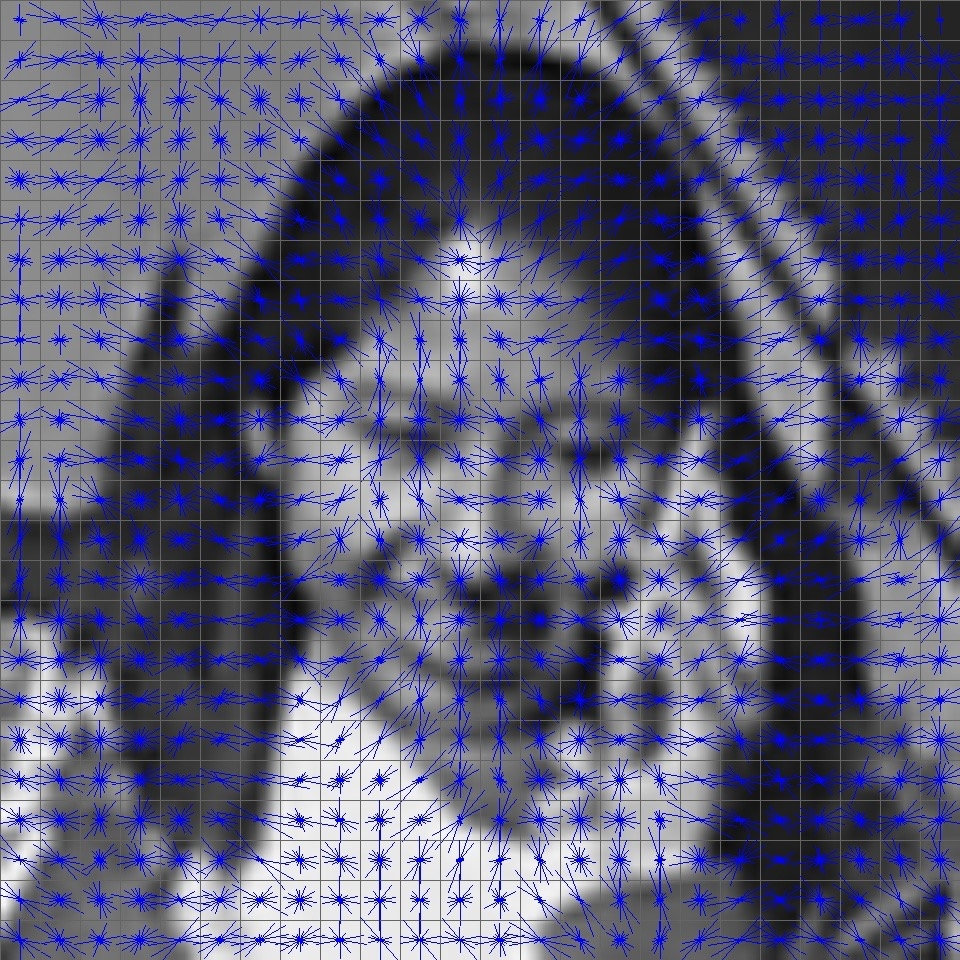
\includegraphics[scale=0.15]{hog}
\caption{Muestra de representación del descriptor de \ac{HOG}(derecha) en una imagen de rostro(izquierda), donde el total de la imagen es transformada a un vector de características.}
\label{im:HOG}
\end{figure}

Para analizar las imágenes representadas por el descriptor de \ac{HOG} se utiliza un \ac{SVM} que se ha sido entrenado con ejemplos positivos y negativos de rostros, con ello se valida los resultados entregados por Viola-Jones vistos en la Figura \ref{im:EscenaViolaResultados}.

Las información proporcionada por el descriptor de \ac{HOG} es entregada a la siguiente parte del proceso como la primera estimación de puntos fiduciales.

%La segunda es que en la continuación de la linea de proceso esta un detector de puntos fiduciales para los rostro detectados, el cual necesita una primera estimación de puntos como lo menciona \cite{baltrusaitis2013constrained} y la representación en el descriptor de \ac{HOG} cumple este trabajo.

\section{Detector de puntos fiduciales}
A partir de los resultados obtenidos por el proceso de detección y validación se tiene una imagen la cual es utilizado en el calculo de los puntos fiduciales mediante \acf{CLNF}.

El método de \ac{EBGM} se basa en modelos de rostros, esto modelos son los puntos encontrados manualmente (ojos, nariz, boca, etc) como se observa en la Figura \ref{im:22Landmark}, dichos modelos se obtienen de un conjunto variado de rostros, a partir de los cuales se calcula un modelo promedio, que se utiliza como estimación inicial para un nuevo rostro mediante el alineamiento con el conjunto de modelos en base a las coordenadas de los ojos 

Se extraen características de la nueva imagen en base a las coordenadas de puntos del modelo promedio, y por cada punto se realiza una comparación del Gabor Wavelet en la nueva imagen con su equivalente en todos los modelos, hasta encontrar el punto del modelo con mayor similitud con ello se obtiene la estimación final de los puntos. Este es un proceso de fundamental ya que una mala estimación de los puntos repercute en el proceso de reconocimiento.

Se propone el uso de \acf{CLNF} en reemplazo de todo el proceso detección de puntos usado en \ac{EBGM}, debido a que \ac{CLNF} es un detector robusto y probado en ambiente no controlados, con una buena tolerancia a variaciones de pose.

\ac{CLNF} recibe el resultado del detector de \ac{HOG} y realiza una estimación de puntos, a partir de ahí se restringe cada punto a un área de vecindad donde se aplica una red neuronal que entrega información espacial sobre cuales son las posiciones que tiene mayor probabilidad de ser el verdadero punto a detectar, el resultado de los puntos detectados es evaluado en conjunto para encontrar la configuración de puntos que resulte mas probable en conjunto, de esta manera se eliminan expresiones y formas de rostro poco probables. Finalmente se entrega las posiciones de 68 puntos en el rostro.

Todo ello permite llevar a \ac{EBGM} a un entorno de vídeo vigilancia sin ayuda de un factor humano, lo que antes no era posible. La totalidad de este proceso se puede apreciar en los algoritmos \ref{alg:Propuesta} y \ref{alg:ImToGrph}.

\section{Pre-procesamiento y normalización de imágenes}\label{scc:PropIluminacion}

Una vez el rostro ha sido detectado, validado y con los puntos fiduciales encontrados, a la imagen del rostro se le aplica una mejora en iluminación a través de ecualización de histograma, transformada de logaritmo y transformada discreta de coseno, presentada en el trabajo de \cite{manjulaimage}, siendo la siguiente Ecuación \ref{f_normaliza}:

\begin{equation}
	F(x,y) = c_{1}*DCT + c_{2}*Lg + c_{3}*HE
    \label{f_normaliza}
\end{equation}
Donde $c_{1}, c_{2}, c_{3}$ son valores tipo peso para equilibrar el efecto de las técnicas usadas, sus valores son de 0.3 , 0.2 y 0.5 respectivamente, donde estos valores fueron calculados después de permutar todos las combinaciones posibles. El resultado de este proceso puede verse en la Figura \ref{im:Preprocess}.

\begin{figure}[h]
\center
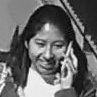
\includegraphics[scale=1.5]{face_original}
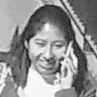
\includegraphics[scale=1.5]{face_pre}
\caption{Muestra del pre-procesamiento aplicado a imágenes, comparando antes y después}
\label{im:Preprocess}
\end{figure}

Junto con ello se aplica el proceso normalización en tamaño que usa \ac{EBGM} que mueve las coordenadas de los ojos a coordenadas pre establecidas $(52, 64)$ y $(76, 64)$ y cambia su resolución a un tamaño de $128 \times 128$ a través de una matriz de transformación de  perspectiva, donde se incluye un borde de 30 pixeles, por lo que el tamaño efectivo de rostros en la imagen final es aproximadamente 90 pixeles de ancho.

Se mantiene la resolución del algoritmo original de \cite{bolme2003elastic} debido a que es necesario aproximarse a resoluciones de rostros que se pueden encontrar en vídeos de vigilancia.
Este proceso y el descrito en la siguiente sección puede ser observado en el algoritmo \ref{alg:ImToGrph}

\begin{algorithm}
\SetKwFunction{ImToGrph}{\textit{ConvertirImagenGrafo}}
\ImToGrph{\var{image},\var{faceLandmark},\var{mask},\var{filter}}\;
{
\var{source} $\gets$ extraer coordenadas de ojos de \var{faceLandmark}\;
\var{M} $\gets$ Calcular una matriz de transformación de perspectiva para que las coordenadas de \var{source} correspondan a las coordenadas $(52,64)$ y $(76,64)$,  y el tamaño de la imagen sea cambiado a $128 \times 128$\;
\var{geo} $\gets$ aplicar la matriz de transformación \var{M} a \var{image}\;
\var{geo} $\gets$ aplicar mejora de iluminación\;
\var{faceLandmark} $\gets$ usar \var{filter} para filtrar puntos fiduciales de interés\;
\var{graph} $\gets$ generar grafo de puntos a partir de \var{faceLandmark}\;
\var{graph} $\gets$ aplicar la matriz de transformación \var{M} a coordenadas de vértices de \var{graph}\;
\ForEach{\var{vertice} en \var{graph}}
{
	extraer Gabor Jet de las coordenadas del vértice usando el conjunto de mascaras de Gabor incluidas en \var{mask}\;
    Almacenar Gabor Jet dentro de \var{graph} en relación con \var{vertice}\;
}
\Return \var{graph}\;
}

\caption{Función para convertir una imagen a Face Graph}
\label{alg:ImToGrph}
\end{algorithm}

\section{Filtro y reajuste de puntos detectados}
Mientras que \ac{EBGM} propuesto en \cite{bolme2003elastic} funciona con 25 puntos fiduciales, de los cuales 3 de ellos se refieren al cabello, usando el detector de puntos \ac{CLNF} se determina 68 puntos de los cuales muchos son cercanos unos a otros por lo que extraer características en todos ellos resulta redundante, ademas ninguno de los puntos obtenidos a través de \ac{CLNF} corresponden a los 3 puntos que se refieren al cabello.

Por lo que es necesario un filtrado de puntos para realizar una correspondencia con los puntos con los que trabaja \ac{EBGM}, por ello se deja de trabajar con estos 3 puntos fiduciales, siendo la cantidad efectiva de trabajo reducida de 25 a 22 puntos, Figura \ref{im:22Landmark}.

\begin{figure}[h]
\center
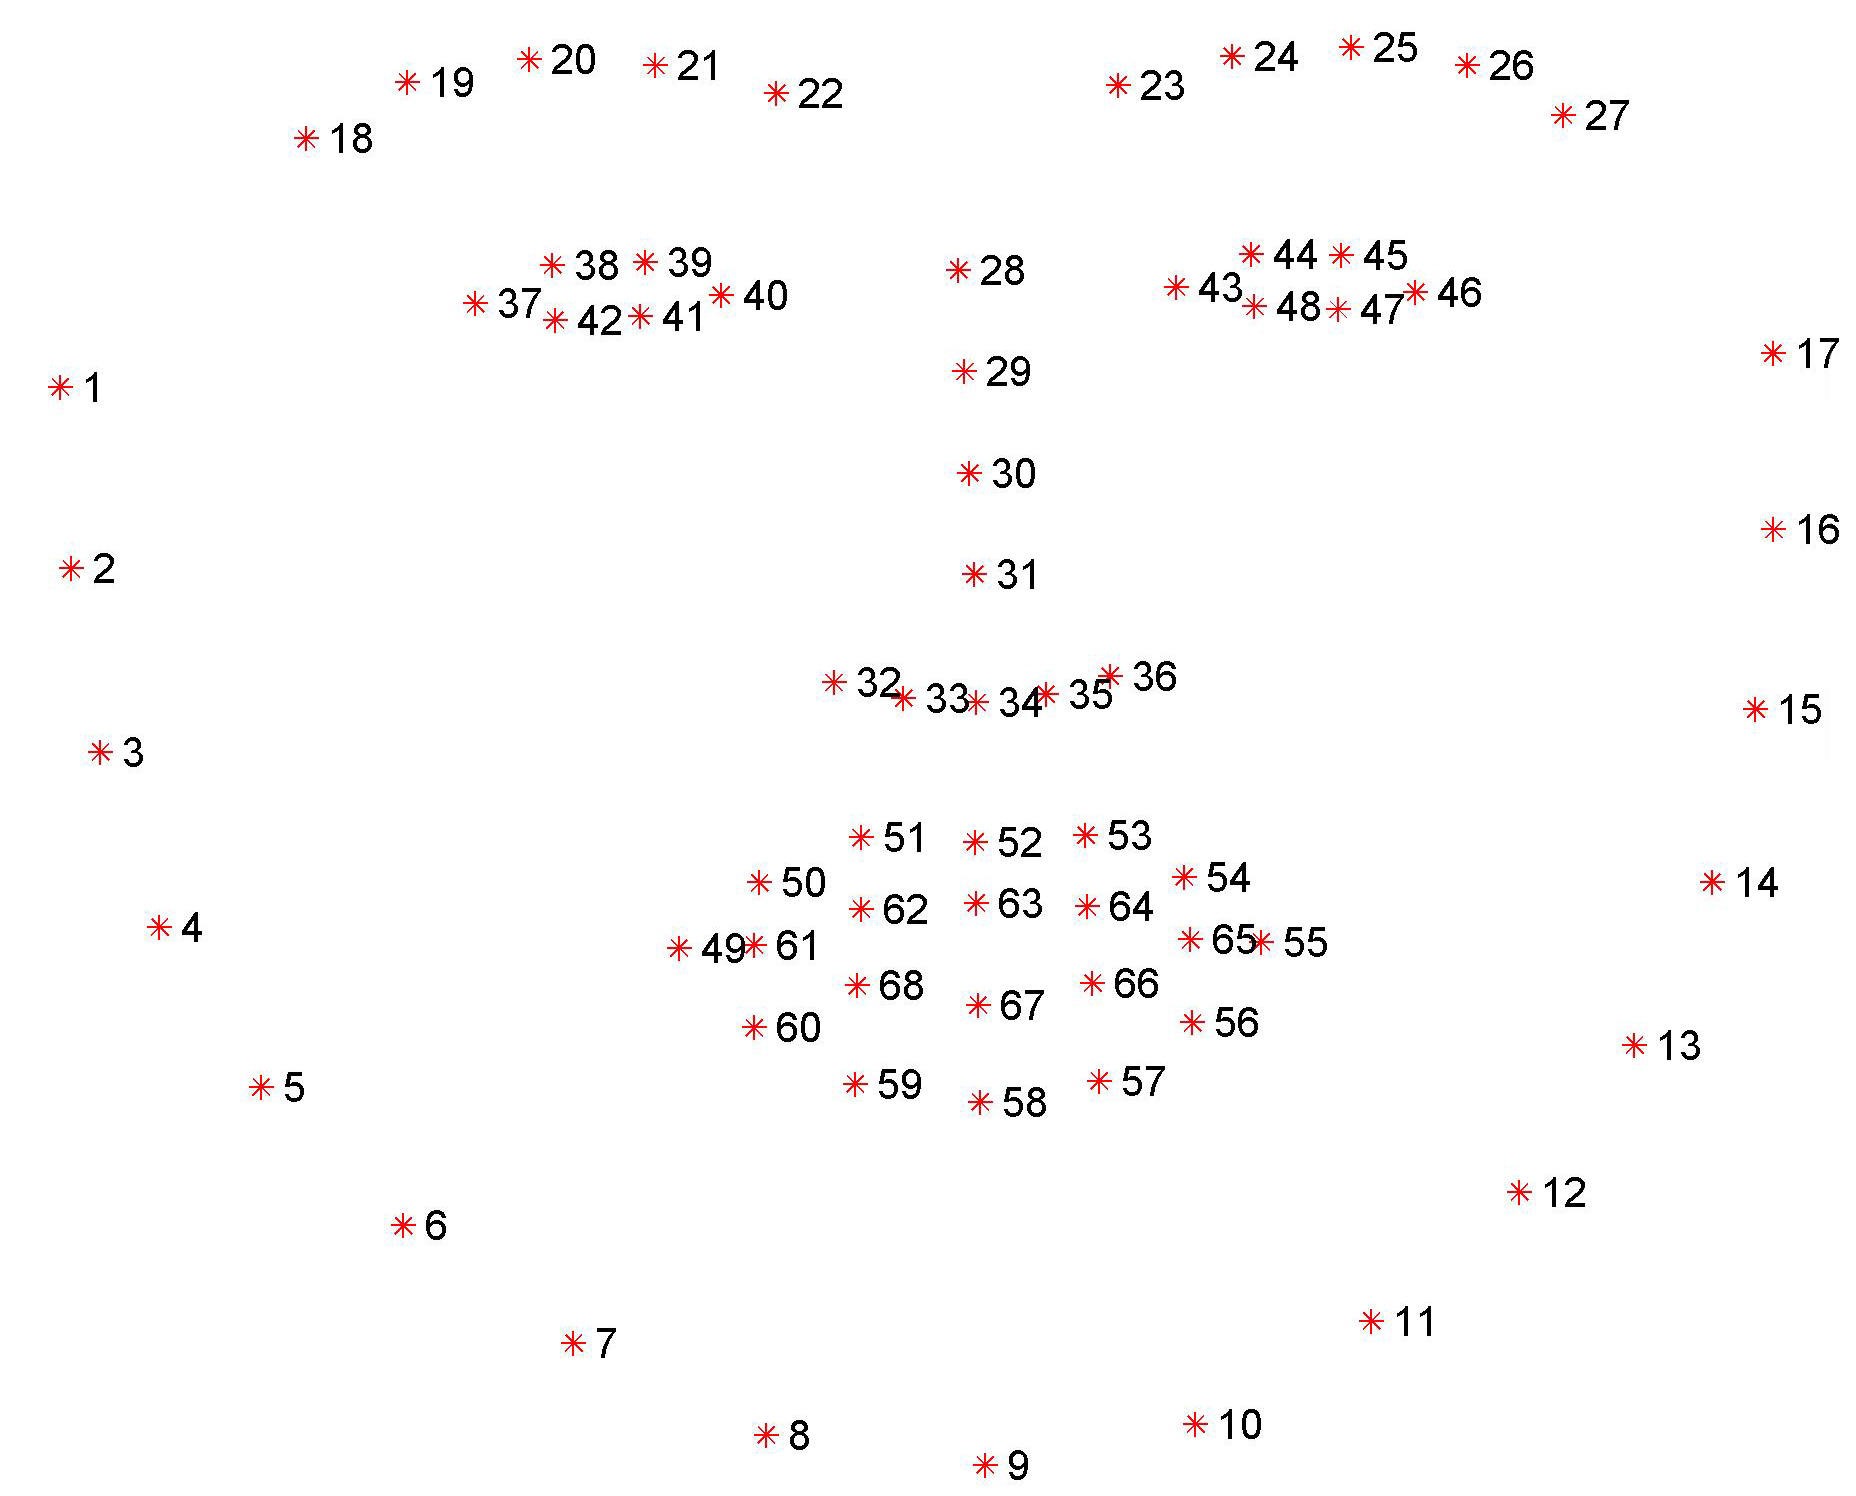
\includegraphics[scale=0.06]{landmarkPoints}
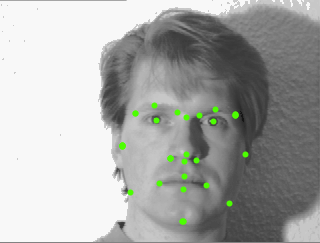
\includegraphics[scale=0.45]{FiltroDespues}
\caption{Izquierda:untos fiduciales entregados por \ac{CLNF}, extraído del proyecto ``Open Face''. Derecha: Puntos fiduciales después del proceso de filtrado}
\label{im:22Landmark}
\end{figure}

Después del filtrado toda la información se completa a un grafo y se aplica una transformada de perspectiva obtenida en el paso anterior para que los vértices correspondan a la imagen normalizada y se continua el proceso de extracción de características de \ac{EBGM}.{}

\section{Proceso de \ac{EBGM}}
Después de reemplazar el proceso de localización de puntos, se continua con el proceso de reconocimiento explicado en la Sección \ref{scc::EBGM} el cual se puede entender en el Algoritmo \ref{alg:ImToGrph}. El proceso empiza cuando extraen características de los puntos fiduciales a través de las convoluciones con las mascaras de Gabor, donde el grupo de coeficientes de resultado son almacenados en una estructura tipo grafo.

Finalmente cada imagen representada como un grafo que es comparada con las imágenes de entrenamiento en una comparación una a uno usando las Ecuaciones \ref{FaceGraphSimiFunc} y \ref{GaborJetSimiFunc}, y eligiendo al grafo con el cual posee mayor similitud. Este proceso es descrito en el Algoritmo \ref{alg:RecFaceGrph}.

Una vez obtenido un resultado de reconocimiento este es visualizado mostrado el nombre del sujeto reconocido sobre el área de su rostro detectado.

\begin{algorithm}
\SetKwFunction{RecFaceGrph}{\textit{ReconocerFaceGraph}}
\RecFaceGrph{\var{faceGraph},\var{graphs}, \var{names}}\;
\var{menor} $\gets$ 10\;
\For{\var{i} $\gets$ 0, \var{i}< tamaño de \var{graphs}}
{
	\var{distance} $\gets$ medir similitud entre \var{faceGraph} y \var{$graphs_{[i]}$}\;
    \If{\var{distance}<\var{menor}}
    {
    	\var{name} $\gets$ \var{$names{[i]}$}\;
    }
}
\Return{name}\;
\caption{Función para comparar un Face Graph con el conjunto de Face Graph de entrenamiento}
\label{alg:RecFaceGrph}
\end{algorithm}

\section{Consideraciones finales}
El aporte de la propuesta es todo el \textit{pipeline} donde se ha logrado aplicar \ac{EBGM} para su uso de vídeo vigilancia gracias al uso de una de las ultimas propuestas en una linea de investigación para el reconocimiento de puntos de interés (\ac{CLNF}), donde el detalle de toda la propuesta puede observarse en la Figura \ref{im:PropPipeline}. 

Se resalta el uso de mejoras para la iluminación usando una unión de varios procesos conocidos, así mismo las transformaciones de tamaño sobre el rostro detectado para poder aproximarnos a resoluciones que son comunes en este escenario particular.

Se realizaron varias pruebas para llegar a la propuesta final, muchas de las cuales demuestran las dificultades que presenta en el reconocimiento de rostros en vídeo vigilancia y la imposibilidad de usar algunas técnicas en este contexto
